\frontmatter % Roman page numbering

\begin{titlepage}
	\begin{center}
	Hochschule Rhein-Waal\\
	Fakutltät Kommunikation und Umwelt\\
	Prof. Dr. Charles Xavier\\
	\vspace{2cm}
	Essay\\
	WS 2015/16\\
	Module: Scientific Writing\\
	\vspace{3cm}
	\uppercase{\textbf{\Large{My Topic}}}\\
	\vspace{8cm}
	My Name (Matriculation Number)\\
	\vspace{1cm}
	Submission Date:\\
	21.01.2016
	\end{center}
\end{titlepage}
\newpage

\addchap*{Abstract}
\lipsum[5]
\textbf{Keywords:}\\
Keyword 1-5
\newpage

\tableofcontents
\newpage

\addchap*{Abbreviations}
\begin{acronym}[rpnx]
	% uppercase letter:
	\acro{URL}{Uniform Resource Locator} 
	% lowercase letter:
\end{acronym}

\lstlistoflistings
\clearpage
\listoftables 
\clearpage
\listoffigures
\clearpage

\mainmatter % Arabic page numbering
\acresetall % if acronyms have been used in the abstract, repeat them.

\chapter{Introduction}
\label{sec:introduction}
\lipsum[1]

\chapter{Main Part}
\label{sec:main}
\lipsum[2] and \ac{URL}

\section{Section A}
\label{sec:a}
\lipsum[3] \autocite{doe2005}

\begin{figure}[ht]
	\centering
    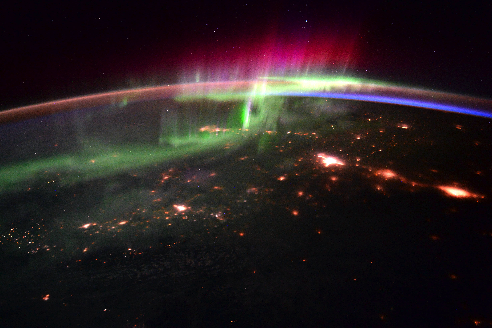
\includegraphics[width=1\textwidth]{figures/aurora.jpg}
	\caption{Aurora and the Pacific Northwest \emph{Image Credits: ESA/NASA}}
	\label{fig:aurora}
\end{figure}

\url{http://www.nasa.gov/image-feature/aurora-and-the-pacific-northwest}

\section{Section B}
\label{sec:b}
\lipsum[4] \textcite{doe2005}

\begin{singlespace}
\begin{lstlisting}[caption=C Hello World, label=lst:hello_world]
#include <stdio.h>

int main(void)
{
	printf("Hello, World\n");
    return 0;
}
\end{lstlisting}
\end{singlespace}

\chapter{Conclusion}
\label{sec:conclusion}
\lipsum[1]

\printbibliography
\appendix
\chapter{Appendix 1}

\newpage
\chapter*{Declaration of Authority}
English\\
I, <name>, hereby declare that the work presented herein is my own work
completed without the use of any aids other than those listed. Any material
from other sources or works done by others has been given due
acknowledgement and listed in the reference section. Sentences or parts of
sentences quoted literally are marked as quotations; identification of other
references with regard to the statement and scope of the work is quoted.
The work presented herein has not been published or submitted elsewhere
for assessment in the same or a similar form. I will retain a copy of this
assignment until after the Board of Examiners has published the results,
which I will make available on request.

German\\
Hiermit erkläre ich, <Name>, dass ich die hier vorliegende Arbeit selbstständig
und ohne unerlaubte Hilfsmittel angefertigt habe. Informationen, die
anderen Werken oder Quellen dem Wortlaut oder dem Sinn nach entnommen
sind, habe ich kenntlich gemacht und mit exakter Quellenangabe
versehen. Sätze oder Satzteile, die wörtlich übernommen wurden, wurden
als Zitate gekennzeichnet. Die hier vorliegende Arbeit wurde noch an
keiner anderen Stelle zur Prüfung vorgelegt und weder ganz noch in
Auszügen veröffentlicht. Bis zur Veröffentlichung der Ergebnisse durch den
Prüfungsausschuss werde ich eine Kopie dieser Studienarbeit aufbewahren
und wenn nötig zugänglich machen.

<Ort, Datum> <Unterschrift>

\backmatter